\section{System Call Interface}
\label{sec:syscall}

\subsection{Lerninhalt}

\begin{itemize}
   \item Sie kennen den Grund, warum es System Calls braucht
   \item Sie kennen den Unterschied zwischen dem User- und dem Kernelmode
   \item Sie kennen die Art, wie System Calls aufgerufen werden
   \item Sie kennen die Interrupt Descriptor Table
   \item Sie kennen den System Call Handler
   \item Sie kennen eine System Call Implementation
   \item Sie kennen den gesamten Ablauf eines System Calls
\end{itemize}

\subsection{System Call}

Nach Abschluss der Bootphase wird der Init-Prozess im \keyword{Usermode} gestartet, welcher alle weiteren Programme
direkt oder indirekt startet. Die Programme lesen und schreiben Dateien im \emph{VFS}. Dabei werden Funktionen der
standard C-Library \keyword{libc} aufgerufen, wie \emph{fopen()}, \emph{fread()} und \emph{fwrite()}. Doch wie sind
diese Funktionen eigentlich Implementiert? \\

Effektiv rufen diese Funktionen einen \keyword{System Call} auf. Der \emph{System Call} wechselt den Prozessormodus
von dem \keyword{Usermode} in den \keyword{Kernelmode}. Das ist notwendig, da nur der \keyword{Kernelmode} direkt Zugriff
auf Hardware hat, um die Stabilität und Sicherheit des Betriebssystems zu gewährleisten.

\subsection{User- und Kernelmode}

Der Unterschied zwischen dem \keyword{Usermode} und dem \keyword{Kernelmode} ist, dass im \keyword{Usermode} nicht alle Instruktionen
des Prozessors aufgerufen werden können. Normalweise macht man nur die Unterscheidungen zwischen diesen beiden Modi, doch der
x86 hat sogar vier unterschiedliche Privilegiestufen. Im Zusammenhang mit den Privilegiestufen redet man oft von \keyword[CPU-Ring]{Ringen}.
Hierbei hat der Ring 0 am meisten und der Ring 3 am wenigsten Rechte (Abbildung \ref{fig:x86_rings}).

\begin{figure}[h!]
   \begin{center}
      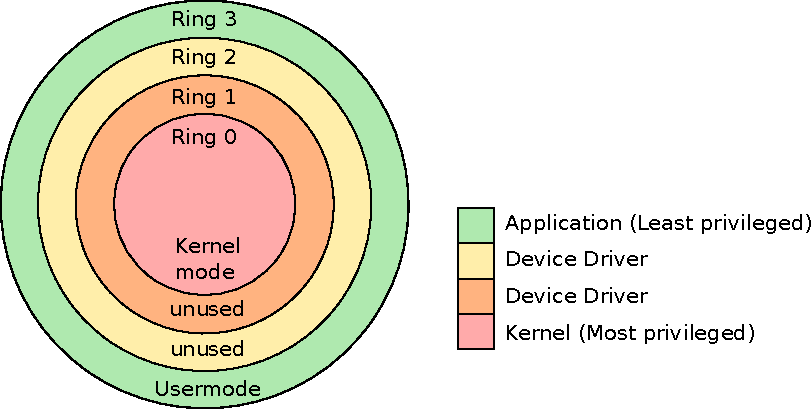
\includegraphics{images/x86_rings}
   \end{center}
   \caption[Ringe des x86]{Ringe des x86\footnotemark}
   \label{fig:x86_rings}
\end{figure} \footnotetext{Bild basiert auf \url{https://en.wikipedia.org/wiki/Protection\_ring}}

Da die Ringe 2 und 3 von keinem üblichen Betriebssystem verwendet werden, unterscheidet man lediglich zwischen User- und Kernelmode.

\subsection{Aufruf eines System Calls}

Um den Schutz der Ringe nicht zu umgehen, ist es nicht möglich aus einem höheren Ring direkt in einen tieferen Ring zu wechseln. Über die
\emph{System Calls} kann jedoch der Kernel aufgerufen werden. Das Listing \ref{x86_syscall} zeigt, wie der System Call \emph{write()} 
unter x86 als Funktion programmiert werden kann.

\begin{lstlisting}[label=x86_syscall,caption=Write system call]
write:
    movl $4,       %eax  ; system call number (3 = read, 4 = write, ...)
    movl 16(%ebp), %ebx  ; arg1: file descriptor to write 
                         ;       (0 = stdin, 1 = stdout, 2 = stderr)
    movl 12(%ebp), %ecx  ; arg2: buffer to be written
    movl 8(%ebp),  %edx  ; arg3: number of bytes to be written
    int  $0x80           ; execute interrupt number 0x80 (linux specific)
\end{lstlisting} \hfill

Die Funktion entspricht folgendem C-Prototyp:
\begin{lstlisting}
int write(int fd, char *buffer, size_t size);
\end{lstlisting} \hfill

Aufrufbar ist die Funktion folgendermassen:
\begin{lstlisting}
char *msg = "Hello world!\n";

int main(int argc, char *argv[]) 
{
   write(STDOUT, msg, strlen(msg));
}
\end{lstlisting} \hfill

Wie im Beispiel ersichtlich ist, wird der System Call über einen Interrupt ausgeführt (\emph{int \$0x80}). Ein solcher Interrupt bewirkt
das gleiche wie wenn die Hardware einen Interrupt auslöst. Das Betriebssystem wird in der Ausführung unterbrochen, wechselt in den 
Kernelmode und führt die \keyword{Interrupt Service Routine} aus. Unter Linux wurde die Interruptnummer 0x80 für System Calls reserviert.
Interrupts, die von Programmen ausgeführt werden können, werden als \keyword{Software-Interrupt} bezeichnet, in Abgrenzung zu den \keyword{Hardware-Interrupts}. 

\subsection{Interrupt Descriptor Table}

Welche Funktion bei einem Interrupt ausgeführt wird, ist abhängig davon, wie die Tabelle names \keyword{Interrupt Descriptor Table (IDT)} ausgefüllt ist. In der IDT können vom Betriebssystem 256
\emph{Interrupt Service Routinen} bestimmt werden. Die Interruptnummer entspricht der Position der ISR. So ist die Interruptnummer 0x80 die 128ste Funktion in der IDT. Die ersten 32 Interruptnummern
sind für Hardwareinterrupts vordefiniert. Dem Betriebsystem steht es frei, die restlichen Interrruptnummern für andere Dinge zu verwenden. Die Tabelle \ref{tab:idt_isr} zeigt den Aufbau der IDT. 

\begin{longtable}{| l | l |} \hline
   \textbf{Interruptnr.} & \textbf{Usage} \\ \hline
   0x00 & Division by zero \\ \hline
   0x01 & Debugger \\ \hline
   0x02 & Non-maskable interrupts (NMI) \\ \hline
   0x03 & Breakpoint \\ \hline
   0x04 & Overflow \\ \hline
   0x05 & Bounds \\ \hline
   0x06 & Invalid Opcode \\ \hline
   0x07 & Coprocessor not available \\ \hline
   0x08 & Double fault \\ \hline
   0x09 & Coprocessor segment overrun \\ \hline
   0x0A & Invalid task state segment \\ \hline
   0x0B & Segment not present \\ \hline
   0x0C & Stack fault \\ \hline
   0x0D & General protection fault \\ \hline
   0x0E & Page fault \\ \hline
   0x0F & Reserved \\ \hline
   0x10 & Math fault \\ \hline
   0x11 & Alignment check \\ \hline
   0x12 & Machine check \\ \hline
   0x13 & SIMD floating-point exception \\ \hline
   0x14 - 0x1F & Reserved \\ \hline
   0x20 - 0xFF & Software interrupts \\ \hline
   \caption{Aufbau der Interrupt Descriptor Table (IDT)}
   \label{tab:idt_isr}
\end{longtable} 

\subsection{Interrupts unter Linux}

Um die Interrupts zu verarbeitet, setzt Linux eigene \emph{Interrupt Service Routinen} in dieser Tabelle fest. In der Datei
\emph{arch/x86/kernel/traps.c} (Listing \ref{idt}) kann diese Zuweisung nachverfolgt werden. Man sieht deutlich die Parallelen zur Tabelle \ref{tab:idt_isr}.
\begin{lstlisting}[caption=arch/x86/include/asm/irq\_vectors.h]
#define SYSCALL_VECTOR                 0x80
\end{lstlisting}

\begin{lstlisting}[label=idt,caption=arch/x86/kernel/traps.c]
void __init trap_init(void)
{
   // ..
   set_intr_gate        (X86_TRAP_DE,         &divide_error                   );
   set_intr_gate_ist    (X86_TRAP_NMI,        &nmi, NMI_STACK                 );
   set_system_intr_gate (X86_TRAP_OF,         &overflow                       );
   set_intr_gate        (X86_TRAP_BR,         &bounds                         );
   set_intr_gate        (X86_TRAP_UD,         &invalid_op                     );
   set_intr_gate        (X86_TRAP_NM,         &device_not_available           );
   set_task_gate        (X86_TRAP_DF,         GDT_ENTRY_DOUBLEFAULT_TSS       );
   set_intr_gate_ist    (X86_TRAP_DF,         &double_fault, DOUBLEFAULT_STACK);
   set_intr_gate        (X86_TRAP_OLD_MF,     &coprocessor_segment_overrun    );
   set_intr_gate        (X86_TRAP_TS,         &invalid_TSS                    );
   set_intr_gate        (X86_TRAP_NP,         &segment_not_present            );
   set_intr_gate_ist    (X86_TRAP_SS,         &stack_segment, STACKFAULT_STACK);
   set_intr_gate        (X86_TRAP_GP,         &general_protection             );
   set_intr_gate        (X86_TRAP_SPURIOUS,   &spurious_interrupt_bug         );
   set_intr_gate        (X86_TRAP_MF,         &coprocessor_error              );
   set_intr_gate        (X86_TRAP_AC,         &alignment_check                );
   set_intr_gate_ist    (X86_TRAP_MC,         &machine_check, MCE_STACK       );
   set_intr_gate        (X86_TRAP_XF,         &simd_coprocessor_error         );
   set_system_intr_gate (IA32_SYSCALL_VECTOR, ia32_syscall                    );
   set_system_trap_gate (SYSCALL_VECTOR,      &system_call                    );
   // ..
}
\end{lstlisting}

Interessant ist vorwiegend diese Zeile:
\begin{lstlisting}
set_system_trap_gate(SYSCALL_VECTOR, &system_call);
\end{lstlisting}

Die Funktion \emph{system\_call()} wird nämlich beim Eintritt des Interrupt \emph{int \$0x80} aus dem Userspace ausgeführt.


\subsection{Interrupt-Handler für den System Call}

Die Aufgabe von \emph{system\_call()} ist es nun, herauszufinden welcher System Call ausgeführt werden soll. Das macht die Funktion über die \emph{System Call Number}, welche per \emph{\%eax}
übergeben wird. Über eine hartcodierte Tabelle namens \emph{System Call Table} findet ein Mapping zwischen der \emph{System Call Number} und der effektiven \emph{System Call} Funktion statt. 
Die Logik hierfür ist in \emph{arch/x86/kernel/entry\_32.S} implementiert. \\

Im voherigem Beispiel wurde für \emph{write()} die Nummer 4 ins Register geschrieben. Das heisst, die Nummer die in \emph{\%eax} liegt, bestimmt was für ein \emph{System Call} durchgeführt
wird. Die anderen Register werden als Parameter verwendet und unterscheiden sich von Funktion zu Funktion.

\subsection{System Call Table}

Im Linux-Kernel 3.2 sind über 300 System Calls definiert. Eine Definition der 
System Calls ist unter \emph{arch/x86/kernel/syscall\_table\_32.S} zu finden. Die Tabelle \ref{tab:x86_syscall} zeigt einen Auszug davon.

\begin{longtable}{| l | l | l | l | l | l |} \hline
   \textbf{Name} & \textbf{\%eax} & \textbf{\%ebx} & \textbf{\%ecx} & \textbf{\%edx} & \textbf{Definiert in}    \\ \hline
   exit          & 1              & int status     &                &                & kernel/exit.c     \\ \hline
   fork          & 2              &                &                &                & arch/x86/kernel/process.c \\ \hline
   read          & 3              & int fd         & void *buf      & size\_t count  & fs/read\_write.c  \\ \hline
   write         & 4              & int fd         & void *buf      & size\_t count  & fs/read\_write.c  \\ \hline
   open          & 5              & char *path     & int flags      &                & fs/open.c         \\ \hline
   close         & 6              & int fd         &                &                & fs/open.c         \\ \hline
   waitpid       & 7              & pid\_t pid     & int *status    & int options    & kernel/exit.c     \\ \hline
   \caption{System Call Tabelle}
   \label{tab:x86_syscall}
\end{longtable}


\subsection{System Call Implementation}

Die Implementierung des System Calls ist einfach. Linux enthält die Macros SYSCALL\_DEFINE0 bis
SYSCALL\_DEFINE6, womit der System Call erstellt wird. Die Zahl am Ende sagt aus, wieviele Parameter
entgegen genommen werden. Das Listing \ref{sys_read} zeigt den Code für den Read-Call.

\begin{lstlisting}[label=sys_read,caption=fs/read\_write.c]
SYSCALL_DEFINE3(read, unsigned int, fd, char __user *, buf, size_t, count)
{
        struct file *file;
        ssize_t ret = -EBADF;
        int fput_needed;

        file = fget_light(fd, &fput_needed);
        if (file) {
                loff_t pos = file_pos_read(file);
                ret = vfs_read(file, buf, count, &pos);
                file_pos_write(file, pos);
                fput_light(file, fput_needed);
        }

        return ret;
}
\end{lstlisting}

\subsection{Ablauf eines System Calls}

Abschliessend soll noch einmal zusammengefasst werden, wie der Ablauf eines System Calls aussieht (Abbildung \ref{syscall_flow}).

\begin{enumerate}
   \item Der Prozess ruft die Libc-Funktion \emph{fread()} auf.
   \item Die Libc führt den System Call \emph{read()} über einen Interrupt aus.
   \item Der Prozessor wechselt in den Kernelmode und entnimmt die ISR in der IDT.
   \item Der Prozessor führt die ISR aus (\emph{system\_call()}).
   \item Die ISR entnimmt den System Call Handler aus der System Call Table.
   \item Die ISR führt den System Call Handler aus (\emph{read()}).
   \item Die ISR gibt den Return über das Register \emph{\%eax} zurück.
   \item Der Prozessor wechselt wieder in den Usermode.
   \item Die Libc gibt den Rückgabewert dem Prozess zurück.
\end{enumerate}

\begin{figure}[h!]
   \begin{center}
      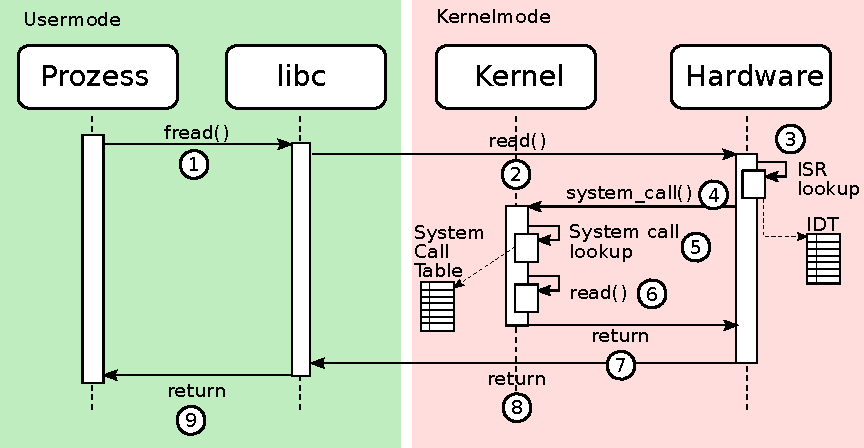
\includegraphics{images/syscall_flow}
   \end{center}
   \caption{Sequenzdiagram eines System Calls}
   \label{syscall_flow}
\end{figure}
\clearpage
\subsection{Zusammenfassung}

\begin{itemize}
   \item Sie kennen den Grund, warum es System Calls braucht
   \item Sie kennen den Unterschied zwischen dem User- und dem Kernelmode
   \item Sie kennen die Art, wie System Calls aufgerufen werden
   \item Sie kennen die Interrupt Descriptor Table
   \item Sie kennen den System Call Handler
   \item Sie kennen eine System Call Implementation
   \item Sie kennen den gesamten Ablauf eines System Calls
\end{itemize}

\summary{
Damit ein Programm eine Funktionalität des Kernels aufrufen kann, muss es einen System Call ausführen. \\

Ein System Call wird über einen Software-Interrupt ausgeführt. Linux unter x86 verwendet hierzu die
Interruptnummer 0x80. \\

Der System Call führt in Normalfall die Libc aus. \\

Tritt ein Interrupt auf, führt der Prozessor die Interrupt Service Routine aus, welche in der Interrupt Descriptor
Table definiert wurde. \\

Die Interrupt Service Routine für den System Call heisst unter Linux system\_call(). \\

Die ISR system\_call() entnimmt aus der System Call Table den System Call Handler und 
führt diesen aus.
}

\subsection{Diskussion}

\begin{itemize}
   \item Wofür braucht es die Ringe in einem Prozessor?
   \item Warum werden die Ringe 2 und 3 von keinem Betriebssystem verwendet?
   \item Was ist der Unterschied zwischen \emph{fread()} und \emph{read()}? Welche Funktion sollte wann verwendet werden?
   \item Kann per \emph{int 0x0E} ein Page fault Interrupt ausgeführt werden?
   \item Unter Linux sind nicht alle der 256 Interrupts implementiert. Was passiert bei einem Aufruf eines nicht definierten Software-Interrupts?
   \item Schauen Sie die System Call Table unter \emph{arch/x86/kernel/syscall\_table\_32.S} durch. Von welchen System Calls haben Sie noch nie
         gehört? Wofür stehen diese?
   \item Wie sind Interrupts in anderen Betriebssystemen implementiert?
\end{itemize}

